\chapter{Consenso di Nakamato}
Prima abbiamo discusso in maniera piuttosto semplicistica come dovrebbe funzionare l'algoritmo di consenso ma, adesso, vediamo chiaramente il perché di alcune specifiche tecniche viste precedentemente.

Ricordiamo che abbiamo bisogno di:
\begin{itemize}
    \item \textbf{Consistenza: }Cioè i nodi onesti devono poter essere d'accordo su quello che è il prossimo blocco da inserire (o quanto meno lo devono essere a lungo termine).
    \item \textbf{Liveness: }Cioè la blockchain deve essere in continua evoluzione.
\end{itemize}
È necessario e lo vedremo tra poco, notare che siamo in un sistema di messaggistico \textbf{asincrono} in cui i messaggi potrebbero non arrivare nello stesso ordine in cui sono stati inviati.

Analizziamo dunque il funzionamento dell'algoritmo di consenso. Come già abbiamo anticipato questo si basa sulla \textbf{Proof of Work}, una sorta di challenge in cui i miner competono per ottenere un hash di un blocco valido che abbia una certa forma dettata da vari zero all'inizio dell'hash. Ogni nodo della rete cercherà di inserire il prossimo blocco all'interno della catena più lunga. Inoltre, vogliamo che in ogni momento che tutti i blocchi a meno degli ultimi k siano considerati \textbf{definitivi.}
Vogliamo dunque ottenere:
\begin{itemize}
    \item \textbf{Consistenza: } Vogliamo che tutti i nodi onesti siano d'accordo su tutti i blocchi a meno degli ultimi k. La probabilità che il k-esimo blocco sia poi sostituito diventa $O(2^{-k})$.
    \item \textbf{Chain Quality: } Qualsiasi sequenza consecutiva di $k$ blocchi contiene "un numero sufficiente di blocchi onesti". I miner che controllano una frazione $p$ della potenza di calcolo mineranno all'incirca una frazione $p$ dei blocchi. Cioè, se i nodi onesti possiedono l'80\% dell'hash power, allora questi dovranno poter creare all'incirca l'80\% dei blocchi della catena.
    \item \textbf{Chain growth: }La catena cresce a un ritmo costante e prevedibile.È la proprietà di Liveness (vitalità) del sistema. Ci garantisce che la blockchain non si "congela" mai. Grazie alla calibrazione automatica della difficoltà dell'hash puzzle, la rete continuerà inesorabilmente a sfornare nuovi blocchi e a processare transazioni indipendentemente da quanti miner si disconnettano o si uniscano alla rete.
\end{itemize}
A questo punto quello che ci viene in mente è, possiamo rendere tutto il processo di mining più veloce? In effetti per come lo abbiamo descritto il sistema è molto lento e per pagare una semplice pizza dovremmo aspettare all'incirca un'ora (cioè che vengano prodotti altri 6 blocchi dopo quello che contiene la nostra transazione) e proprio questo fa' sì che la nostra moneta sia poco utilizzabile nel caso di un utilizzo in questo tipo di contesto.

Immaginiamo uno scenario in cui un attaccante cerchi di generare una catena alternativa per annullare una transazione passata, attacco noto come \textbf{Selfish Mining}. Supponiamo che il destinatario della transazione attenda $z$ blocchi (conferme) prima di considerare il pagamento definitivo. A questo punto, l'attaccante parte con uno svantaggio di $z$ blocchi rispetto alla catena onesta.
\begin{figure}[H]
    \centering
    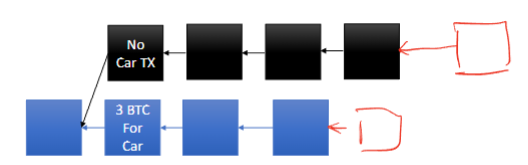
\includegraphics[width=0.5\linewidth]{Images/capitolo_3/tentativo_ds.png}
\end{figure}


Definiamo le seguenti probabilità:
\begin{itemize}
    \item $p$: la probabilità che il prossimo blocco venga minato dai nodi onesti.
    \item $q$: la probabilità che il prossimo blocco venga minato dall'attaccante.
\end{itemize}
Ad ogni nuovo blocco scoperto, il divario tra le due catene varia: aumenta di $1$ se vince la rete onesta, diminuisce di $1$ se vince l'attaccante. A vince se riesce a raggiungere il target z. \\
La probabilità $P_z$ che l'attaccante riesca, prima o poi, a colmare il deficit di $z$ blocchi e a superare la catena onesta è data dalla formula:
\[
P_z = 
\begin{cases} 
1 & \text{se } q \ge p \\
\left(\frac{q}{p}\right)^z & \text{se } p > q 
\end{cases}\]
Questa equazione ci fornisce due dimostrazioni cruciali sul funzionamento di Bitcoin:
\begin{enumerate}
    \item \textbf{Vulnerabilità al 51\%:} Se l'attaccante possiede la maggioranza dell'hash power ($q \ge p$), la probabilità di successo è $1$ (certezza assoluta). Anche se non ci dice nulla riguardo a quanto tempo sia necessario per farlo.
    \item \textbf{La regola delle 6 conferme:} Se i nodi onesti sono in maggioranza ($p > q$), la probabilità di successo dell'attaccante decade in modo esponenziale all'aumentare di $z$. Ad esempio, persino contro un attaccante formidabile che controlla il 30\% della rete ($q = 0.3$), se si attendono $z = 6$ blocchi, la probabilità che l'attacco vada a buon fine scende a circa lo $0.6\%$. Per questo motivo, attendere 6 conferme rende la transazione statisticamente irreversibile.
\end{enumerate}
\section{Dimostrazione Matematica dell'attacco}

Per ricavare la formula del \textit{Nakamoto Consensus}, poniamoci l'obiettivo di trovare $P_1$, ovvero la probabilità che l'attaccante recuperi uno svantaggio di esattamente $1$ blocco.

Poiché il recupero di ogni singolo blocco è un evento indipendente, la probabilità di recuperare uno svantaggio di $z$ blocchi è semplicemente:
$$P_z = (P_1)^z$$

Per calcolare $P_1$, definiamo l'evento $A$ come "l'attaccante riesce a recuperare lo svantaggio" e l'evento $F$ come "il prossimo blocco viene minato dall'attaccante" (mentre $\neg F$ indica che viene minato dai nodi onesti).
Possiamo calcolare la probabilità totale di $A$ dividendo lo spazio degli eventi:
$$P_1 = \Pr[A] = \Pr[A \cap F] + \Pr[A \cap \neg F]$$

Applicando la definizione di probabilità condizionata, possiamo espandere la formula:
$$P_1 = \Pr[A \mid F]\Pr[F] + \Pr[A \mid \neg F]\Pr[\neg F]$$

Analizziamo i singoli termini sapendo che la probabilità di successo dell'attaccante è $q$ e quella della rete onesta è $p$:
\begin{itemize}
    \item $\Pr[F] = q$
    \item $\Pr[\neg F] = p$
    \item $\Pr[A \mid F] = 1$: se l'attaccante trova il blocco, il deficit si azzera subito e ha recuperato con certezza.
    \item $\Pr[A \mid \neg F] = P_2$: se i nodi onesti trovano il blocco, il deficit passa da $1$ a $2$. La probabilità di recuperare da $2$ è $P_2$, che sappiamo essere uguale a $(P_1)^2$.
\end{itemize}

Sostituendo i valori nell'equazione otteniamo:
$$P_1 = 1 \cdot q + (P_1)^2 \cdot p$$

Riordinando i termini, arriviamo a un'equazione di secondo grado nell'incognita $P_1$:
$$p(P_1)^2 - P_1 + q = 0$$

Risolvendo questa equazione (e ricordando l'identità $p + q = 1$), si ottengono direttamente due possibili soluzioni:
$$P_1 = 1 \quad \text{oppure} \quad P_1 = \frac{q}{p}$$

Poiché $P_1$ è una probabilità, il suo valore deve essere $\le 1$. 
Se l'attaccante ha la maggioranza dell'hash power ($q \ge p$), la frazione $q/p$ sarebbe $\ge 1$, rendendo $P_1 = 1$ l'unica soluzione logicamente accettabile (la frode avrà sicuramente successo).
Se invece i nodi onesti sono in maggioranza ($p > q$), la teoria dei processi stocastici ci impone di considerare la radice strettamente minore, portandoci alla conclusione finale:
$$
P_1 = 
\begin{cases} 
1 & \text{se } q \ge p \\
\frac{q}{p} & \text{se } p > q 
\end{cases}
$$
\subsection{La scelta della Difficoltà e il Network Delay}

Alla luce delle garanzie di sicurezza offerte dal \textit{Nakamoto Consensus}, sorge spontanea una domanda: se il sistema è sicuro finché la maggioranza della potenza è onesta, perché imporre una difficoltà tale da generare un blocco solo ogni $10$ minuti? Perché non abbassare il parametro di difficoltà per confermare le transazioni in pochi secondi?

La risposta risiede nei limiti fisici dell'infrastruttura di rete, in particolare nella \textbf{latenza di propagazione} (\textit{Network Delay}), indicata con $\Delta$.

In una rete P2P globale, quando un nodo trova un blocco, necessita di un tempo $\Delta$ affinché questo venga trasmesso e verificato da tutti gli altri peer. Durante questo lasso di tempo, i nodi onesti che non hanno ancora ricevuto l'aggiornamento continuano a impiegare potenza di calcolo per risolvere un blocco ormai obsoleto. L'energia spesa in questo gap $\Delta$ è di fatto \textbf{sprecata}. Al contrario, un avversario malevolo fortemente centralizzato non subisce latenze interne, ottimizzando il 100\% del suo \textit{hash rate}.

\subsubsection{Il Discount Rate della potenza onesta}
Possiamo modellare matematicamente l'impatto di questo spreco definendo i seguenti parametri:
\begin{itemize}
    \item $n$: numero totale di nodi nella rete.
    \item $\alpha$: frazione dei nodi che si comportano onestamente (dunque vi sono in totale $\alpha n$ nodi onesti).
    \item $p$: probabilità che un \textit{singolo} nodo risolva il puzzle crittografico in un dato round.
\end{itemize}

Vogliamo trovare la probabilità che la rete onesta nel suo complesso trovi un blocco in un singolo round. Per farlo, passiamo dall'evento complementare: la probabilità che \textbf{nessun} nodo onesto trovi il blocco è $(1-p)^{\alpha n}$. 
Dunque, la probabilità che \textbf{almeno un} nodo onesto ci riesca è:
$$ 1 - (1-p)^{\alpha n} $$
Poiché in Bitcoin la probabilità $p$ di trovare un hash valido è infinitesimamente piccola, possiamo applicare l'approssimazione binomiale (o sviluppo di Taylor al primo ordine, per cui $(1-x)^k \approx 1 - kx$ per $x \to 0$):
$$ 1 - (1-p)^{\alpha n} \approx 1 - (1 - \alpha n p) = \alpha p n $$

Questa espressione, $\alpha p n$, rappresenta la probabilità di successo per round dell'intera rete onesta. Di conseguenza, il tempo atteso (in round) per la scoperta di un nuovo blocco è semplicemente il suo inverso:
$$ \frac{1}{\alpha p n} $$

Poiché per ogni blocco trovato si "perdono" $\Delta$ round per la propagazione, l'efficienza reale della rete onesta è data dal rapporto tra il tempo di lavoro utile e il tempo totale impiegato (lavoro utile + spreco):
$$ \text{Efficienza} = \frac{\frac{1}{\alpha p n}}{\frac{1}{\alpha p n} + \Delta} = \frac{1}{1 + \alpha p n \Delta} \approx 1 - \alpha p n \Delta $$

Questo fattore agisce come \textbf{Discount Rate} sulla potenza reale degli onesti. La potenza effettiva a disposizione dei nodi corretti non è più $\alpha n$, ma diviene:
$$ (1 - \alpha p n \Delta) \alpha n $$

Se la difficoltà del puzzle fosse troppo bassa, i blocchi verrebbero trovati troppo frequentemente, rendendo il parametro $\Delta$ dominante. Il \textit{discount rate} abbatterebbe drasticamente l'efficacia dei nodi onesti, generando continue biforcazioni e avvantaggiando gli attaccanti centralizzati. Per mantenere la stabilità e la sicurezza, Satoshi Nakamoto ha calibrato la difficoltà affinché il tempo atteso per un blocco ($10$ minuti, ovvero $600$ secondi) sia di ordini di grandezza superiore al tempo di latenza globale della rete $\Delta$ (pochi secondi), minimizzando così lo spreco di risorse.

\subsection*{Condizione di sicurezza}
Nei sistemi distribuiti tradizionali, il consenso si basa sul conteggio dei nodi ("Un nodo, un voto") e la tolleranza viene espressa in base al numero di partecipanti malevoli (es. si tollerano al massimo $1/3$ di nodi disonesti). 
In una rete non centralizzata come Bitcoin, questo approccio fallirebbe istantaneamente a causa del \textbf{Sybil Attack} poiché un singolo attaccante potrebbe generare milioni di nodi virtuali a costo zero, acquisendo artificialmente la maggioranza dei voti.

Per neutralizzare questo vettore di attacco, la Proof of Work sposta il paradigma di voto da \textit{"Un nodo, un voto"} a \textit{"Una CPU (un hash), un voto"}.
Di conseguenza, il protocollo Bitcoin \textbf{può tollerare un numero teoricamente infinito di nodi disonesti}, a un'unica condizione: che la somma della loro potenza computazionale (\textit{Hash Power}) rimanga strettamente minoritaria rispetto a quella dei nodi onesti ($q < p$). Nelle analisi matematiche e statistiche del protocollo, parametri come la probabilità di successo $p$ non rappresentano la percentuale di utenti onesti, ma la frazione di potenza di calcolo globale sotto il loro controllo.

\subsection{Vantaggi e Svantaggi}
Il sistema a consenso di Nakamoto presenta alcuni vantaggi tra cui:
\begin{itemize}
    \item \textbf{Partecipazione anonima e facile accesso:} Poiché è possibile partecipare semplicemente con l'indirizzo pubblico della chiave generata, è chiaro che la partecipazione sia "anonima" anche se di questo parleremo dopo. Sempre per lo stesso motivo, poiché generare chiavi è estremamente semplice, è di facile accesso e, quindi, molto scalabile.
    \item \textbf{Impossibile prevedere il vincitore:} Se il sistema fosse prevedibile, ci dovremmo trovare ad avere a che fare con casi di collusioni in cui si cerca di corrompere il leader per fargli inserire o non inserire certe transazioni. Invece, poiché il vincitore non è prevedibile, questo non è chiaramente uno scenario fattibile.
    \item \textbf{Tolleranza di tanti nodi malevoli: }Per quanto detto prima, fintanto che la potenza di calcolo dei nodi malevoli è inferiore rispetto alla potenza di calcolo dei nodi onesti, vi è una grossa tolleranza.
\end{itemize}
Come tutte le cose belle, però, abbiamo alcuni svantaggi parecchio ovvi che riguardano principalmente il fatto che questo metodo è \textbf{lento} e, quindi, non permette pagamenti immediati e, a causa delle proof-of-work, abbiamo un \textbf{grosso dispendio energetico} rendendo, di fatto, il consumo di energia tra i più alti rispetto perfino ad alcuni paesi del mondo.
